\problemname{Divide the Ducks Equally}
\noindent

As the benevolent ruler of POland, you want all your citizens to be happy. 
It is therefore deeply concerning that two children are quarreling. 
Specifically, they are arguing over $2N$ kodsport-ducks that are scattered 
across a plane, and the children disagree about how many ducks each should get.

To resolve the conflict, you need to create a crack in the ground — a straight 
line that divides the plane into two parts. The crack must be placed so that 
exactly $N$ ducks end up on each side, ensuring that both children receive 
the same number of ducks. Each duck is located at an integer coordinate.

Since you prefer simplicity and elegance, your crack will be a straight line of the form $y = kx + m$, where $k$ and $m$ may be \textbf{decimal numbers}.\\
If such a line exists that divides the ducks equally, output it.\\
Otherwise, print ``impossible''.

\section*{Input}
The first line contains an integer $N$ ($1 \leq N \leq 10^5$), where $2N$ is the total number of ducks.

The following $2N$ lines describe the ducks' positions. Each line contains two integers $x_i, y_i$ ($0 \leq x_i, y_i \leq 10^6$), the coordinates of the $i$-th duck.
All ducks have unique positions.

\section*{Output}
If it is possible to divide the ducks equally, output two real numbers $k$ and $m$ that describe the line $y = kx + m$.
$k$ and $m$ may contain at most 50 characters each. It is guaranteed that the judge will make calculations exactly with $k$ and $m$.
Note that your program might round $k$ and $m$ when they are printed. \\
The answer will be accepted if the line divides the ducks into two equally sized groups. If multiple solutions exist, you may output any of them.\\
If a duck is exactly on the line, it is considered to be below the line.

If it is impossible to divide the ducks equally, print ``impossible''.

\section*{Scoring}
Your solution will be tested on a set of test groups, each worth a number of points. Each test group contains
a set of test cases. To get the points for a test group you need to solve all test cases in the test group.

\noindent
\begin{tabular}{| l | l | p{12cm} |}
  \hline
  \textbf{Group} & \textbf{Points} & \textbf{Constraints} \\ \hline
  $1$    & $15$       & $N = 1$ \\ \hline
  $2$    & $15$       & $x_i = 0$ for all ducks. \\ \hline
  $3$    & $15$       & $x_i \leq 1$ for all ducks. \\ \hline
  $4$    & $15$       & $N = 2$ \\ \hline
  $5$    & $20$       & $N \leq 1000$ \\ \hline
  $6$    & $20$       & No additional constraints. \\ \hline
\end{tabular}

\section*{Explanation of Samples}
In each of the following images, all ducks are marked as black dots. The crack used in the sample solution is represented as a red line.
Note that there are multiple valid solutions in all cases.

\begin{centering}
  \begin{figure}[h]
      \centering
      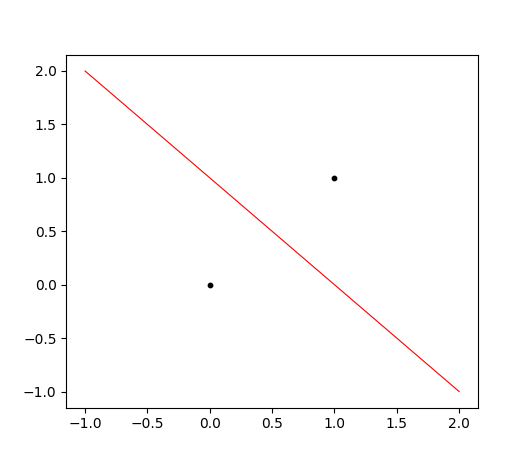
\includegraphics[width=0.3\textwidth]{sample1.png}
      \caption{The image represents the first sample.}
      \label{fig:enter-label}
  \end{figure}
\end{centering}

\begin{centering}
  \begin{figure}[h]
      \centering
      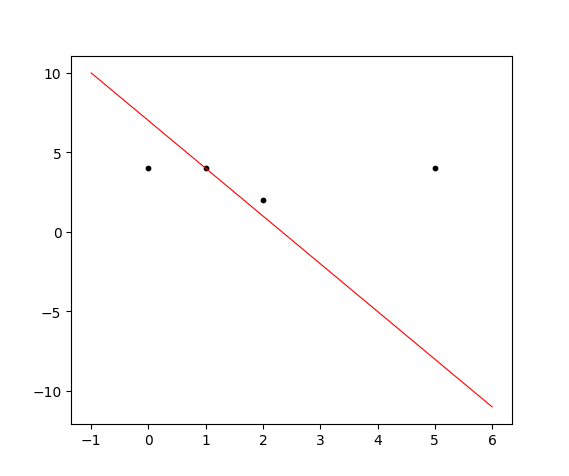
\includegraphics[width=0.3\textwidth]{sample2.png}
      \caption{The image represents the second sample. It is hard to see, but the second point
      is just below the line.}
      \label{fig:enter-label}
  \end{figure}
\end{centering}

\begin{centering}
  \begin{figure}[h]
      \centering
      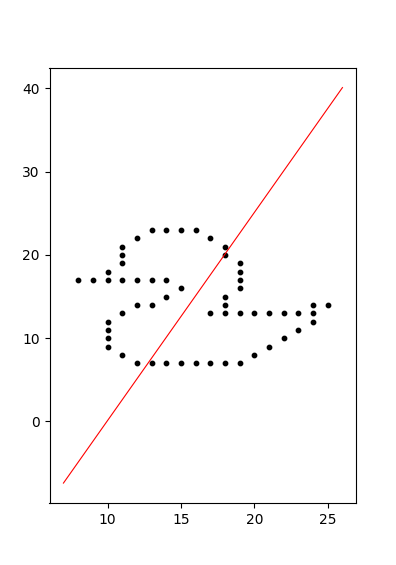
\includegraphics[width=0.3\textwidth]{sample3.png}
      \caption{The image represents the third sample.}
      \label{fig:enter-label}
  \end{figure}
\end{centering}
